\documentclass[Journal,letterpaper,NoLists]{ascelike-new}
\usepackage{amsmath,amssymb}
\usepackage{booktabs}
\usepackage{graphicx}
\usepackage{multirow}
\usepackage[figurename=Fig.,labelfont=bf,labelsep=period]{caption}
\usepackage{url}
\usepackage[colorlinks=true,citecolor=black,linkcolor=black,urlcolor=blue]{hyperref}
\setlength{\emergencystretch}{3em}

\newcommand{\fcntm}{FC-NTM}

\NameTag{Wang, \today}

\begin{document}

\title{Field-Cooperative Neural Topic Modeling of Civil Engineering Literature:
Missing-Abstract Inference}

\author[1]{Hongli Wang}
\author[1]{Qingpeng Man}

\affil[1]{School of Civil Engineering, Harbin Institute of Technology, Harbin, China.
E-mails: 2010254508@qq.com (H.~Wang); manqp@126.com (Q.~Man, corresponding author)}

\maketitle

\begin{abstract}
Title--abstract records are a core form of civil engineering literature, and part of most
collections is available with titles only. This paper studies how the two fields of such a record
should be modelled together, and what can still be inferred when the abstract is missing. We
present FC-NTM, a field-cooperative neural topic model that builds one conditional variational
stream per field, shares a single topic decoder across the streams, and handles partial and
complete field absence with cross-field reconstruction, a consistency term and field-level word
masking; a single trained model yields a native beta read-out and a class TF-IDF read-out under
one evaluation vocabulary. On civil engineering title-abstract records from OpenAlex (6000/2000),
FC-NTM attains the highest coherence among the evaluated methods and read-out configurations, and
a ten-seed paired comparison against BTM favours it in all ten seeds (plus 0.049 class TF-IDF
read-out and plus 0.061 native beta read-out, a raw-parameter read-out whose batch-normalised
counterpart is smaller). Title-only routing reaches 0.66 accuracy against OpenAlex primary-topic labels on the subset
covered by the fifteen selected topics (42.9\% of the test split); these labels are assigned
automatically and serve as an external reference rather than expert-annotated ground truth, and
the task is a routing aid complementing, rather than replacing, supervised classification. A same-budget concatenated-field control is close on
every corpus, so the reported gains pertain to the complete modelling configuration, and the
occlusion experiments characterise inference stability under missing-field conditions when read
alongside absolute prediction loss and topic agreement. The results establish a corpus-dependent
empirical case for field-cooperative topic modelling and identify the conditions that require
further validation. Cross-domain evaluations and read-out protocols are reported in the paper and
supplement, and per-seed results, fixed data splits and hyper-parameters are released with the
code.
\end{abstract}

\KeyWords{topic model; field cooperation; neural variational inference; fielded documents with short summary fields; class TF--IDF read-out; complementarity measures}

\section{Introduction}

Topic models summarise unlabelled collections as readable topic structures and are widely used in
news, software repositories and social media analysis. In many of these collections a record is not
a homogeneous bag of words but a pair of fields with different functions: a title that gives a
highly compressed summary, and a body that supplies context, motivation and qualifications. The
same topic is expressed differently in the two fields -- the body side tends to carry context and
causes, the summary side tends to carry objects and actions. Civil and construction engineering
records are a natural instance: bibliographic title--abstract pairs, technical specifications and
contract clauses, and accident reports all pair a short summary-like field with a longer contextual
field. Topic modelling of such documents is useful both for literature navigation and for records
whose long field is unavailable, for example when only titles have been collected.

Topic modelling has moved from probabilistic graphical models to neural variational models. LDA is
the classical bag-of-words Bayesian model \cite{blei2003lda}; GSDMM addresses short texts with a
collapsed Gibbs Dirichlet--multinomial mixture \cite{yin2014gsdmm}; AVITM introduces a linear
decoder into a variational auto-encoder and defines the LDA and ProdLDA generative processes
\cite{srivastava2017avitm}; NVDM applies variational auto-encoders to text early on
\cite{miao2016nvdm}; CTM/CombinedTM combine contextual sentence embeddings with bag-of-words
counts \cite{bianchi2021ctm}; ETM defines topics in a word-embedding space \cite{dieng2020etm};
BTM models word pairs instead of document-level counts and remains a strong baseline for short
texts \cite{yan2013btm}. Surveys note that structured and short-text corpora are still open
problems for neural topic models \cite{wu2024survey}.

Existing neural topic models exploit the internal field structure of a document only to a limited
degree: the fields are usually concatenated into one bag of words and their division is discarded.
Multi-view and multi-source topic modelling has been explored for parallel corpora, multiple data
sources and cross-modal settings
\cite{kurle2019multisource,zhang2017robust,pergola2021disentangled,liu2022dualview}; structured
neural topic models for reviews encode user--item context and assign words to sentence-level
aspects \cite{esmaeili2019structured}; structural topic models describe metadata with
document-level covariates \cite{roberts2019stm}. Short-text work such as DV-BTM optimises two
views jointly \cite{liu2022dualview}, CRNTM reinforces topic
inference with context \cite{crntm2020}, and DVI-DTM learns dual-view representations for
interpretable dynamic topics \cite{dvidtm2026}. In these works the two views play known roles
(query--document, user--item, or aspect layers); the setting studied here differs: the two fields
of the \emph{same} record are modelled by separate variational streams, and their relation is
fixed by the record schema rather than inferred as an explicit latent variable.  Separate
encoders, posterior alignment and missing-view inference are building blocks adopted from this
literature; the contribution claimed here is the field-cooperative configuration and its
read-out protocol, not those building blocks themselves.

In engineering informatics, text mining has become a recognised analysis tool: content analysis and
classification of safety reports \cite{civilsafety2015,civilaccident2018}, automated classification
of regulations and contracts and extraction of contractual risk clauses
\cite{compliance2013,ontology2015,contract2022,risknlp2023}, and surveys of natural language processing for
construction \cite{civilnlp2021,civilnlp2023}. Topic models have entered the field as well: DUET
applies LDA topic modelling to social-media text for detecting physical events in urban areas
\cite{duet2019}, neural topic modelling has
been used to map machine-learning applications in buildings \cite{civiltopic2024}, and semantic
topic modelling has been used to build taxonomies for digital building passports \cite{passport2026}. In contrast to
these works, we do not treat the topic model as a feature extractor for a downstream classifier.
We study the \emph{internal} field structure of an engineering record: topic inference when a field
is missing, field-restricted read-out, and whether these read-outs can be measured reliably.

This paper makes two contributions. \textbf{Methodologically}, it proposes the field-cooperative
neural topic model \fcntm{}, which models the two fields of a record as two conditional variational
streams that share one linear topic decoder, adds cross-field reconstruction and a field
consistency regulariser, and handles partial and complete field absence with field-level word
masking and whole-field dropout; a single trained model yields both a decoder $\beta$ read-out and
a class TF--IDF read-out under a unified evaluation vocabulary. \textbf{Empirically}, the paper characterises the conditions under which field-cooperative topic
modelling provides reproducible read-out gains, and how inference behaves when a field is missing.
On the civil corpus and on GitHub issues (background/summary length ratio 12.9) and AG News (3.9)
we extend \fcntm{} and BTM to ten seeds: both read-outs favour \fcntm{} on the civil corpus
($+0.049$ class TF--IDF and $+0.061$ $\beta$ $C_V$, 10/10 seeds), the class TF--IDF read-out is
$+0.028$ $C_V$ above BTM on GitHub (95\% CI $[+0.012,+0.043]$, 9/10 seeds) and $-0.009$ on AG News
(CI includes zero, 3/10), while on the two public corpora the $\beta$ read-out is lower than BTM.
We therefore claim the multi-seed-supported read-out advantages on the civil corpus and on GitHub,
and report the absence of an advantage on AG News. Two field-relation measures
are tested as candidate predictors -- a held-out mutual-prediction score and a post-training
occlusion diagnostic -- and neither serves as a monotone criterion. The value of field cooperation
is thus restricted to reproducible field-restricted read-outs and to the behaviour of inference
under missing fields, not to an unconditional performance advantage.

\section{Related Work}

\noindent\textbf{Neural topic models.} Neural topic models map a bag of words to a latent Gaussian posterior and decode topics from it:
NVDM applied variational auto-encoders to text \cite{miao2016nvdm}, ProdLDA introduced a linear
decoder with a readable topic--word matrix \cite{srivastava2017avitm}, CTM/CombinedTM concatenate
sentence embeddings with counts \cite{bianchi2021ctm}, and ETM defines topics in an embedding space
\cite{dieng2020etm}. For short texts, BTM models word pairs \cite{yan2013btm}, BERTopic and Top2Vec
build representations from class TF--IDF statistics and joint embeddings
\cite{grootendorst2022bertopic,angelov2020top2vec}, GraphBTM and BCK-TM add word-pair structure
\cite{zhu2018graphbtm,zhang2020bcktm}, and BigARTM provides an additive regularisation framework
\cite{vorontsov2015bigartm}. Our decoder follows the ProdLDA structure with topic orthogonality,
dropout \cite{srivastava2014dropout} and validation-based early stopping \cite{prechelt1998early};
training loops and learning rates differ between models, so the objectives are not identical
across algorithms.

\noindent\textbf{Multi-view and structured-document topic models.} Multi-view topic models share information across views: bilingual, multi-source and disentangled
models \cite{kurle2019multisource,zhang2017robust,pergola2021disentangled,liu2022dualview},
structured neural topic models for reviews \cite{esmaeili2019structured}, metadata-conditioned
models \cite{card2018metadata,roberts2019stm}, and dual-view short-text work (DV-BTM, CRNTM and
DVI-DTM) \cite{liu2022dualview,crntm2020,dvidtm2026}, alongside related word-pair models
\cite{relationalbtm2018,sparsebtm2021}. Multi-source variational inference with per-source encoders
and posterior-divergence terms \cite{kurle2019multisource} and JMVAE, which infers a missing
modality from the remaining one \cite{suzuki2017jmvae}, already contain separate encoders,
posterior alignment and missing-view inference; SubNTM models sub-document topics
\cite{nguyen2026subntm}. Our setting is fixed by the record schema: two textual fields share one
vocabulary and one linear decoder, and the study asks what field-restricted read-outs and
missing-background inference measure rather than claiming these building blocks as new.

\noindent\textbf{Text mining and topic modelling of engineering documents.} Engineering informatics has an extensive text-mining literature on safety reports
\cite{civilsafety2015,civilaccident2018}, regulatory and contractual documents
\cite{compliance2013,ontology2015,contract2022,risknlp2023}, and domain surveys
\cite{civilnlp2021,civilnlp2023}. Topic models include DUET \cite{duet2019}, neural topic modelling
of building applications \cite{civiltopic2024} and passport taxonomies \cite{passport2026}. These
studies use topics as inputs to classification or mapping; we study the field structure inside one
engineering record and ask when field-restricted topics and missing-field inference are
informative.

\section{Method}

Figure~\ref{fig:arch} gives an overview of \fcntm{}. The two fields are encoded by separate
conditional variational streams that share one topic decoder; the streams are tied by cross-field
reconstruction and a consistency term, and field-level masking with whole-field dropout covers
partially and fully missing fields.

\begin{figure}[t]
\centering
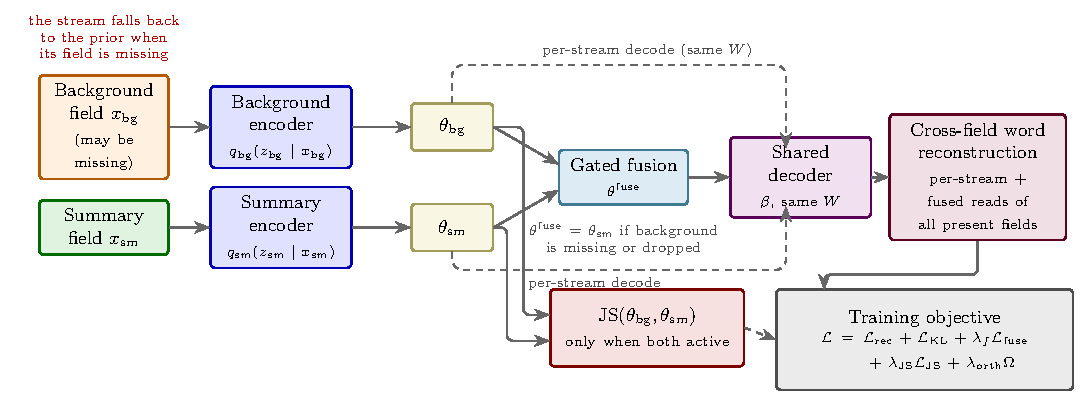
\includegraphics[width=0.98\textwidth]{fig_architecture_en.pdf}
\caption{Overview of \fcntm{}. Each field has its own conditional variational stream. Solid arrows
show the fused path, in which the gated mixture is decoded and every present field is reconstructed;
dashed arrows show the per-stream decodes, which reuse the same decoder parameters. The training
objective combines per-stream reconstruction, the KL terms of the active streams, fused
reconstruction, the JS term (computed only when both streams are active) and the topic-orthogonality
penalty. A missing or dropped field falls back to the prior, so the gated mixture reduces to the
remaining stream ($\theta^{\mathrm{fuse}}=\theta_{\mathrm{sm}}$ when the background field is missing
or dropped). The native $\beta$ read-out uses the
raw matrix $W$, whereas generation follows the batch-normalised path of Eq.~\eqref{eq:decode}.}
\label{fig:arch}
\end{figure}

\noindent\textbf{Problem setting.} Each record $d$ consists of field A (\emph{background}, e.g.\ the abstract of a paper or the body
of an issue) and field B (\emph{summary}, e.g.\ the title), with $N$ records in total and a shared
evaluation vocabulary of $V$ terms. The model maintains $K$ topics, a document--topic distribution
$\theta_d\in\Delta^{K-1}$, and a topic--word matrix $\beta\in\mathbb{R}^{K\times V}$ shared by both
fields. The task is to infer $\theta_d$ and $\beta$ from unlabelled records, to produce readable
topics in two read-outs, and to remain usable when one field is partially or entirely missing at
inference time.

\noindent\textbf{Field streams and the shared decoder.} Each field is encoded by its own two-layer MLP encoder (200 hidden units, Softplus activations,
dropout $0.2$) into the parameters of a field-conditioned Gaussian posterior,
\begin{equation}
q_f(z_f\mid x_f)=\mathcal N\big(\mu_f(x_f),\operatorname{diag}(\sigma_f^2(x_f))\big),
\qquad f\in\{\mathrm{bg},\mathrm{sm}\},
\end{equation}
where $x_f$ is the $L_1$-normalised bag of words of field $f$ and $\log\sigma_f^2$ is capped at
$2$. Posterior means are mapped to topic proportions by a deterministic softmax,
$\bar\theta_f=\operatorname{softmax}(\mu_f(x_f))$, which is used at evaluation time in place of
sampling; $\bar\theta_f$ is therefore a deterministic topic-proportion estimate, not the
expectation of $\operatorname{softmax}(z_f)$. Both streams share one linear topic--word matrix
$W\in\mathbb{R}^{K\times V}$, and write $\theta_f\in\mathbb{R}^{1\times K}$ for the topic
proportions of field $f$ under the row-vector convention,
\begin{equation}
p(w\mid\theta_f)=\operatorname{softmax}\!\big(\mathrm{BN}(\theta_f W)\big),
\label{eq:decode}
\end{equation}
where $\theta_f$ passes through dropout before the product, $\mathrm{BN}$ is a batch-normalisation
layer \emph{without} affine parameters applied over the vocabulary dimension (batch statistics
during training, running statistics at evaluation), and there is no additive bias. The $\beta$
read-out of the ``Unified topic-word read-out'' subsection reads the raw rows of $W$, whereas generation uses the
normalised path of Eq.~\eqref{eq:decode}; the gap between the two is quantified in the
Supplementary Material.

\noindent\textbf{Training objective.} For a document $d$ let $\mathcal{G}_d$ collect its present fields (the background field is present
when the record carries it; the summary stream is always instantiated, including zero-vector
inputs after preprocessing) and let
$\mathcal{A}_d\subseteq\mathcal{G}_d$ be the \emph{active streams}, i.e.\ present fields whose
stream is not removed by whole-field dropout. Write $n^{(g)}_{dw}$ for the raw count of word $w$
in field $g$. Each active stream decodes once (Eq.~\eqref{eq:decode}) and reconstructs
\emph{every present field},
\begin{equation}
R_f=\sum_{g\in\mathcal{G}_d}\omega_g\,R_f(g),\qquad
R_f(g)=-\sum_{w=1}^{V} n^{(g)}_{dw}\,\log p\!\left(w\mid\theta_f\right),
\label{eq:recon}
\end{equation}
with fixed field weights $\omega_{\mathrm{bg}}=2.0$ and $\omega_{\mathrm{sm}}=1.0$. The summary
stream therefore reconstructs the background field as well (cross-field reconstruction), and a
background field that was observed but dropped during training stays in the reconstruction
targets even though its own stream is inactive, whereas a naturally missing background field
enters neither the inputs nor the targets. The per-document objective is
\begin{equation}
\mathcal{L}_d=\frac{1}{|\mathcal{A}_d|}\sum_{f\in\mathcal{A}_d}
\Big[R_f+\lambda_{\mathrm{KL}}(t)\,\mathrm{KL}_f\Big]
+\lambda_f R_{\mathrm{fuse}}+\lambda_{\mathrm{JS}}\,\mathrm{JS},
\label{eq:total}
\end{equation}
where $\mathrm{KL}_f=\mathrm{KL}\big(q_f(z_f\mid x_f)\,\|\,\mathcal N(0,I)\big)$ is summed over
the $K$ latent dimensions and clamped at zero, and $\lambda_{\mathrm{KL}}(t)=0.05\min(1,t/20)$
anneals linearly during the first 20 epochs. The fused term
$R_{\mathrm{fuse}}=\sum_{g\in\mathcal{G}_d}\omega_g R_{\mathrm{fuse}}(g)$ is a second
reconstruction of both present fields from the fused topic mixture
\begin{equation}
\theta_d^{\mathrm{fuse}}=g\,\theta_{\mathrm{bg}}+(1-g)\,\theta_{\mathrm{sm}},
\qquad g=\sigma(w),\quad w\in\mathbb{R},
\label{eq:lfuse}
\end{equation}
for records with both fields present, and
$\theta_d^{\mathrm{fuse}}=\theta_{\mathrm{sm}}$ when the background field is missing or
dropped. During training Eq.~\eqref{eq:lfuse} combines the \emph{sampled} per-stream
proportions that also feed the per-stream reconstructions; at inference time, and for the JS
term below, the deterministic estimates $\bar\theta_f$ are used instead, so at inference
Eq.~\eqref{eq:lfuse} is a convex combination of two deterministic topic-proportion estimates,
which is why we call it a \emph{fused topic mixture} rather than a posterior. The gate
$g$ receives gradients only through $R_{\mathrm{fuse}}$, so with $\lambda_f=0$ the model
degenerates exactly to fixed mean fusion. The consistency term
\begin{equation}
\mathrm{JS}=\tfrac12\,\mathrm{KL}\!\big(\bar\theta_{\mathrm{bg}}\|m\big)
+\tfrac12\,\mathrm{KL}\!\big(\bar\theta_{\mathrm{sm}}\|m\big),
\qquad m=\tfrac12\big(\bar\theta_{\mathrm{bg}}+\bar\theta_{\mathrm{sm}}\big),
\end{equation}
acts on the deterministic topic proportions, not on the Gaussian posteriors, and is computed only
for documents whose two streams are both active, so no record is implicitly regularised more
strongly than another. A topic-orthogonality penalty keeps the rows of $W$ apart,
\begin{equation}
\Omega=\frac{1}{K(K-1)}\sum_{k\neq k'}\big|\cos\langle W_k,W_{k'}\rangle\big|,
\end{equation}
and the batch objective is $\frac{1}{|B|}\sum_{d\in B}\mathcal{L}_d
+\lambda_{\mathrm{orth}}\Omega$ with $\lambda_{\mathrm{orth}}=0.2$.

Two masking mechanisms expose the model to missing fields, and they act on different units.
(i) \emph{Word-level input dropout} (denoising) is applied during training to the bag-of-words
\emph{word types} of each field: each BoW dimension is independently zeroed with probability
$0.30$ (background) or $0.40$ (summary) in the encoder view only, while the reconstruction
targets remain the complete counts. (ii) \emph{Whole-field dropout} removes the background stream
of each training document with probability $0.5$ and substitutes the prior; the summary stream is
never dropped and learns to reconstruct both fields on its own. The test-time occlusion protocol
of the ``Field inference under partial occlusion'' subsection instead masks \emph{token positions} in the raw field text, so the
training and evaluation units should not be conflated. The consistency weight
$\lambda_{\mathrm{JS}}=0.5$, the fusion weight $\lambda_f=0.5$ and the dropout probabilities were
selected on held-out data.

\noindent\textbf{Optimisation.} Training uses Adam (learning rate $5\times10^{-4}$, momentum parameters $0.9$ and $0.999$),
mini-batches of $128$, gradient-norm clipping at $5.0$ and a budget of $700$ epochs. After the KL
warm-up the state with the lowest held-out loss is kept, for which $20\%$ of the training split is
held out; the patience is $150$ epochs. Evaluation-mode inference is deterministic: the
reparameterisation sampling is switched off and the held-out loss uses posterior means.
Numerical-anomaly recovery rolls the weights back to the most recent finite epoch, clears the
optimiser moments and halves the learning rate; this recovery step is separate from the
best-held-out-epoch selection of the early-stopping loop.

\noindent\textbf{Unified topic-word read-out.} \label{sec:readout}

Topic-word comparisons are only meaningful if every model is read out with the same vocabulary and
the same number of words per topic. We therefore fix one evaluation vocabulary and exactly ten
words per topic. The \textbf{$\beta$ read-out} takes the top ten words of each normalised row of
the model's topic--word matrix; for \fcntm{} these are the raw rows of $W$, whereas generation
uses Eq.~\eqref{eq:decode}. LDA, BTM, NMF, ProdLDA, ETM, CTM-lite, CombinedTM and \fcntm{} are all
evaluated this way. The \textbf{class TF--IDF read-out} aggregates the training-term counts by the
soft document--topic assignment of the model, applies a BERTopic-style class TF--IDF transform,
and then takes the top ten words; for \fcntm{} this read-out is built from the fused topic mixture
$\bar\theta^{\mathrm{fuse}}$, which is why the two read-outs can rank models differently. The
sensitivity of the raw-parameter read-out relative to the generative read-out is reported in the
Supplementary Material.

\section{Experiments}

\noindent\textbf{Corpora and evaluation protocol.} We use three dual-field corpora. The \textbf{civil engineering corpus} is the application corpus:
title--abstract records of English journal articles from OpenAlex \cite{openalex2022} (\url{https://openalex.org}) in \emph{Civil and Structural
Engineering} and \emph{Building and Construction} (2000--2023, CC-licensed records only), 6000
training and 2000 test records, with the title as the summary field and the abstract as the
background field (mean length ratio 11.2). \textbf{GitHub issues} \cite{openindex2026} pairs the
issue body with its title (four mature repositories, 6000/2000, ratio 12.9), and \textbf{AG News}
\cite{zhang2015char} pairs the description
with the headline (6000/7600, ratio 3.9). All corpora are lower-cased and tokenised on letter
sequences; stop words and very short tokens are removed, the vocabulary is built from the training
split only, and test records never enter the vocabulary. Table~\ref{tab:civil} reports the
application corpus and Tables~S14 and~S15 the two public corpora, all on
the same evaluation vocabulary with exactly ten words per topic and $K=30$. The evaluation
protocol (vocabulary, ten words per topic, coherence and
diversity metrics) is shared by every model, whereas the training procedure differs across
algorithm families and is described in the ``Baselines, training protocols and metrics'' subsection. Because a 400-record
development subset was used during design, every result is also
recomputed on a development-free test subset (1600 GitHub and 7200 AG News records); the
re-scoring removes direct test overlap only and cannot undo the model selection that already
happened, so it is reported as a sensitivity analysis rather than as an untouched confirmation
set. The results are organised around three questions: how well civil title--abstract records can
be structured into verifiable topics; how much signal remains when the abstract is missing; and
how much the complete field-cooperative configuration adds over a concatenated single-encoder
control. Cross-corpus diagnostics support these questions rather than replacing them.

\noindent\textbf{Baselines, training protocols and metrics.} \label{sec:protocol}

Baselines are LDA \cite{blei2003lda}, BTM \cite{yan2013btm}, NMF with a KL objective
\cite{lee2001nmf}, ProdLDA \cite{srivastava2017avitm}, ETM \cite{dieng2020etm}, CTM-lite, the
official CombinedTM \cite{bianchi2021ctm}, BERTopic \cite{grootendorst2022bertopic} and Top2Vec
\cite{angelov2020top2vec}; contextual models use Sentence-BERT embeddings
\cite{reimers2019sbert}. The implementations fall into four families with different training
procedures, which we do not describe as interchangeable loops: Gibbs sampling (BTM, LDA), matrix
factorisation (NMF), neural variational models (ProdLDA, ETM, CTM-lite and \fcntm{} share the Adam
loop and the 700-epoch budget but differ in learning rate; the official CombinedTM keeps its own
loop), and embedding clustering (BERTopic, Top2Vec), which choose their own topic numbers and are
shown for reference only. Full hyper-parameters are listed in the Supplementary Material. Quality
is measured by $C_V$ coherence \cite{roder2015coherence}, NPMI \cite{bouma2009npmi,lau2014tea}, UCI
and UMass, IRBO topic diversity \cite{webber2010rbo} and a $K$-corrected exclusivity
$EXCL_{KADJ}$ \cite{bischof2012exclusivity}; topics with non-finite scores are dropped, so the
effective topic count is recorded next to every score.

 \begin{table}[t]
\centering
\caption{Topic quality on the civil engineering corpus (unified evaluation vocabulary, ten words per topic; values are means over seeds 11/23/37, and the training procedure differs across algorithm families as described in the ``Baselines, training protocols and metrics'' subsection; BERTopic and Top2Vec choose their own topic numbers and are shown for reference).}
\label{tab:civil}
\small
\begin{tabular}{lcccccc}
\toprule
Model & Topics & $C_V$ & NPMI & UMass & EXCL$_{\mathrm{KADJ}}$ & IRBO \\
\midrule
BTM & 30 & 0.583$\pm$0.010 & 0.128$\pm$0.009 & $-$2.18 & 0.283 & 0.944 \\
CombinedTM & 30 & 0.539$\pm$0.029 & 0.082$\pm$0.028 & $-$6.11 & 0.063 & 0.998 \\
\fcntm{}-cTFIDF & 30 & \textbf{0.636}$\pm$0.014 & \textbf{0.159}$\pm$0.011 & $-$2.21 & 0.165 & 0.937 \\
\fcntm{} & 30 & 0.633$\pm$0.014 & 0.154$\pm$0.022 & $-$2.85 & 0.014 & 0.990 \\
ETM & 30 & 0.581$\pm$0.012 & 0.119$\pm$0.007 & $-$2.75 & 0.379 & 0.963 \\
ProdLDA & 30 & 0.580$\pm$0.023 & 0.125$\pm$0.017 & $-$3.84 & 0.051 & 0.999 \\
Top2Vec & 153 & 0.515$\pm$0.002 & 0.029$\pm$0.011 & $-$8.52 & 0.359 & 0.995 \\
NMF & 30 & 0.598$\pm$0.009 & 0.135$\pm$0.006 & $-$2.86 & 0.559 & 0.984 \\
BERTopic & 29 & 0.576$\pm$0.026 & 0.116$\pm$0.027 & $-$5.06 & 0.563 & 0.991 \\
CTM-lite & 30 & 0.536$\pm$0.030 & 0.098$\pm$0.027 & $-$3.85 & 0.013 & 0.995 \\
LDA & 30 & 0.554$\pm$0.008 & 0.056$\pm$0.025 & $-$4.62 & 0.602 & 0.987 \\
\bottomrule
\end{tabular}
\end{table}

\noindent\textbf{Main results.} On the civil engineering corpus (Table~\ref{tab:civil}), \fcntm{} attains the highest coherence
among all evaluated models under both read-outs ($C_V=0.633$ for the $\beta$ read-out and $0.636$ for
the class TF--IDF read-out; NPMI $0.154$ and $0.159$ over seeds 11/23/37), ahead of NMF (0.598),
BTM (0.583) and the neural baselines, and the ten-seed extension keeps both read-out advantages
(Table~\ref{tab:seed-paired}); Figure~\ref{fig:seedpaired} shows the per-seed differences behind
these means, including the corpora where the advantage is not observed.
Figure~S1 summarises the model-by-model comparisons under both coherence metrics.
On AG News, \fcntm{}-cTFIDF reaches $C_V=0.612$ and NPMI $=0.173$, above BTM under the matched
class TF--IDF read-out ($0.593$ / $0.169$) and clearly above the $\beta$ read-outs of ProdLDA,
ETM, NMF, CTM-lite and LDA; under its own $\beta$ read-out BTM keeps a small lead ($0.600$ versus $0.586$). On GitHub issues, \fcntm{}-cTFIDF reaches $C_V=0.727$ and NPMI $=0.274$,
above BTM at both read-outs ($0.712$ / $0.232$ for the native $\beta$ read-out, $0.700$ / $0.235$
matched), and above the sentence-embedding baselines (CombinedTM $0.643$, BERTopic $0.540$).
The matched-read-out advantage over BTM is therefore $+0.027$ $C_V$ and $+0.039$ NPMI on GitHub and
$+0.019$ / $+0.004$ on AG News for three seeds, but the per-seed structure differs: on GitHub all
three seeds are positive, whereas the AG News mean is carried by two of three seeds and the NPMI
advantage by one. On the development-free test subset the ordering is unchanged
(GitHub $0.734$ versus $0.711$, NPMI $0.284$ versus $0.248$; AG News $0.610$ versus $0.590$, NPMI
$0.172$ versus $0.167$; with BTM's native $\beta$ read-out, $0.734$ versus $0.726$ and $0.610$
versus $0.598$).

\begin{figure}[t]
\centering
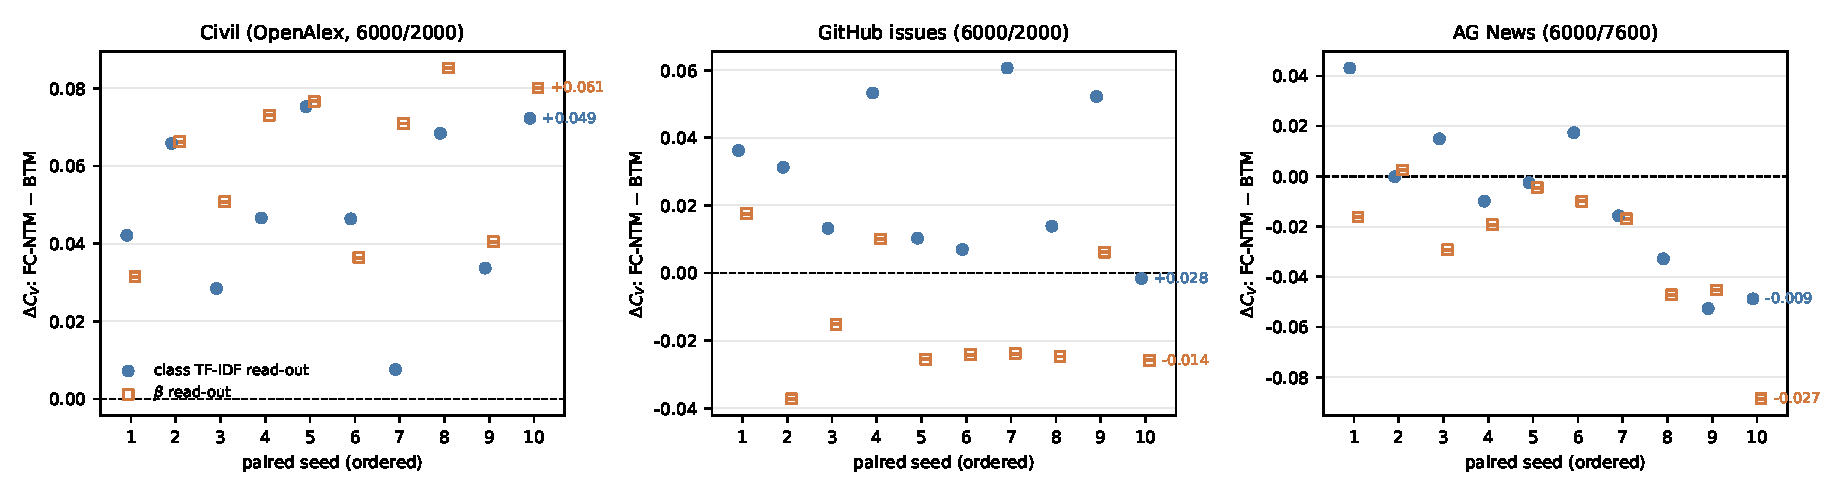
\includegraphics[width=0.98\textwidth]{fig_seed_paired_en.pdf}
\caption{Per-seed paired comparison of \fcntm{} and BTM (ten seeds per corpus, $C_V$). Each point
is one paired seed: filled circles show the class TF--IDF read-out and open squares the $\beta$
read-out, and the dashed horizontal line marks the BTM level (zero difference). The class
TF--IDF read-out is positive throughout on the civil corpus and on GitHub issues, while the AG
News seeds are mixed, which is the corpus-dependent pattern the mean differences summarise.}
\label{fig:seedpaired}
\end{figure}

\noindent\textbf{Read-out-matched comparison.} Table~S16 collects the read-out-matched comparison across models and read-outs.

The class TF--IDF read-out depends on the model and the corpus: on GitHub it lifts CTM-lite,
ProdLDA and LDA by $0.091$, $0.087$ and $0.068$ but leaves ETM and NMF unchanged or worse, while on
AG News it helps every model except BTM. Comparisons therefore use the matched read-out. Under it,
\fcntm{}-cTFIDF leads the strongest GitHub baselines (BTM $0.700$, CTM-lite $0.675$, ETM $0.669$,
ProdLDA $0.666$) by $0.027$--$0.061$ $C_V$ and $0.039$--$0.059$ NPMI, larger than its seed-to-seed
standard deviation ($0.022$); on AG News the advantage over BTM is $+0.019$ $C_V$ but rests on two
of three seeds, and under the native $\beta$ read-out \fcntm{} is below BTM ($0.586$ versus
$0.600$); on the civil corpus NMF ($0.607$) and ETM ($0.603$) are ahead of BTM ($0.590$), and
\fcntm{}-cTFIDF leads them by $0.029$ and $0.033$ $C_V$, although the ten-seed comparison is
against BTM. Two caveats remain: the TF--IDF transform does not automatically favour BTM
($0.712	o0.700$ on GitHub, $0.600	o0.593$ on AG News), and the architecture hyper-parameters
of \fcntm{} were selected on development data while the baselines use defaults.

\noindent\textbf{Ten-seed paired comparison.} To test whether the three-seed differences are seed noise, we extend \fcntm{} and BTM to ten seeds
on all three corpora (adding 53/71/89/101/113/127/139) and compare both read-outs and the
occlusion behaviour seed by seed; the occlusion rows use pre-selected baselines (BTM on all three
corpora and additionally LDA on AG News) rather than a full tournament.

\begin{table}[t]
\centering
\caption{Ten-seed paired comparison of \fcntm{} and BTM on the three corpora. The read-out rows report $C_V$ differences (\fcntm{} minus BTM at the same read-out); the occlusion rows compare the relative degradation $\mathrm{NLL}(100\%)/\mathrm{NLL}(25\%)$, so a positive value means \fcntm{} is more stable. The occlusion rows use the pre-selected baselines (BTM on all three corpora and additionally LDA on AG News) rather than a full baseline tournament. CIs are two-sided 95\% $t$ intervals; sign and Wilcoxon tests are two-sided.}
\label{tab:seed-paired}
\footnotesize
\setlength{\tabcolsep}{3pt}
\begin{tabular}{@{}llcccccc@{}}
\toprule
Corpus & Comparison & Mean diff. & CI low & CI high & Positive & Sign $p$ & Wilcoxon $p$ \\
\midrule
GitHub & Class TF--IDF & $+$0.028 & $+$0.012 & $+$0.043 & 9/10 & 0.021 & 0.004 \\
GitHub & $\beta$ read-out & $-$0.014 & $-$0.028 & $-$0.001 & 3/10 & 0.344 & 0.037 \\
GitHub & Occlusion (vs.\ BTM) & $+$0.024 & $+$0.022 & $+$0.026 & 10/10 & 0.002 & 0.002 \\
\midrule
AG News & Class TF--IDF & $-$0.009 & $-$0.030 & $+$0.013 & 3/10 & 0.344 & 0.375 \\
AG News & $\beta$ read-out & $-$0.027 & $-$0.047 & $-$0.008 & 1/10 & 0.021 & 0.004 \\
AG News & Occlusion (vs.\ BTM) & $+$0.025 & $+$0.024 & $+$0.026 & 10/10 & 0.002 & 0.002 \\
AG News & Occlusion (vs.\ LDA) & $-$0.013 & $-$0.014 & $-$0.012 & 0/10 & 0.002 & 0.002 \\
\midrule
Civil corpus & Class TF--IDF & $+$0.049 & $+$0.033 & $+$0.064 & 10/10 & 0.002 & 0.002 \\
Civil corpus & $\beta$ read-out & $+$0.061 & $+$0.047 & $+$0.075 & 10/10 & 0.002 & 0.002 \\
Civil corpus & Occlusion (vs.\ BTM) & $-$0.003 & $-$0.004 & $-$0.002 & 0/10 & 0.002 & 0.002 \\
\bottomrule
\end{tabular}
\end{table}

Four observations follow. First, the matched read-out advantage on GitHub survives ten seeds:
\fcntm{}-cTFIDF is $+0.028$ $C_V$ above BTM (95\% CI $[+0.012,+0.043]$, 9/10 seeds positive) and
its relative degradation advantage is $+0.024$ (10/10, $p=0.002$). Second, the civil corpus gives
the largest and most consistent read-out advantage: $+0.049$ class TF--IDF and $+0.061$ native
$\beta$ $C_V$ (the latter refers to the raw-parameter read-out; the BN-generated counterpart
is smaller, see the Supplementary Material), both with all ten paired differences positive
($p=0.002$), although the occlusion
ratio still favours BTM ($-0.003$, 0/10). Third, the three-seed AG News advantage is not replicated under ten seeds: the matched read-out difference is $-0.009$, with a confidence interval that includes zero (3/10). Fourth, on the
two public corpora the native $\beta$ read-out is below BTM ($-0.014$ and $-0.027$); overall the
advantage is corpus-dependent and read-out-dependent: largest on the civil corpus under both
read-outs, moderate and class-TF--IDF-focused on GitHub, and neutral on AG News. Confidence intervals
describe training (and masking) randomness under a fixed corpus and a fixed design; the $p$-values
are exploratory and not corrected for multiple comparisons.

\noindent\textbf{Field redundancy and the gain.} Table~S8 reports the held-out redundancy measures together with the observed
gains, and Figure~S2 relates them across the two public corpora.

The redundancy measures are fitted on the training split and evaluated on the test split. The two
corpora have almost the same held-out predictability (GitHub is slightly higher,
$\rho^2_{\mathrm{cca}}$ 0.306 versus 0.245), while \fcntm{}-cTFIDF is slightly above BTM on both at
three seeds ($+0.027$ and $+0.019$ matched) and the ten-seed extension keeps the difference on
GitHub ($+0.028$, 9/10) and turns it negative on AG News ($-0.009$, 3/10); the civil corpus,
whose redundancy is not measured here, shows the largest extension advantage
(Table~\ref{tab:seed-paired}). The evidence
therefore supports neither ``complementary fields gain'' nor ``redundant fields pay a price''. The
differences (0.019--0.027 matched, 0.012--0.014 against BTM's native $\beta$ read-out) are of the
same order as the seed-to-seed variation, so they are described as a small advantage over BTM
rather than as a significant improvement. The occlusion diagnostic
points in the same direction: both corpora change coherence by almost nothing
(GitHub $+0.009\pm0.022$, AG News $+0.018\pm0.013$). We therefore do not use field redundancy as a
predictor of the gain; establishing such a criterion would require calibration on more corpora and
an independent test corpus.

\noindent\textbf{Field inference under partial occlusion.} \label{sec:occl}

The central mechanism is field complementarity: when part of field A is unavailable, a model should
use the still visible field B to recover the missing content. The protocol (Supplementary Material)
masks a fraction $p$ of the background-field tokens in the test documents, re-infers the topic
proportions from the remaining input, and scores the occluded tokens under the model's own word
distribution; it reports the per-token NLL, the agreement of the most probable topic with the
unoccluded inference, and the posterior JS divergence. Every model uses its own inference path and
its own word distribution, so no cross-model read-out convention is involved. When a document has
no visible evidence at all, BTM and NMF fall back to the training-corpus topic prior instead of
treating a zero vector as a distribution, which would inflate the NLL to $\log 10^{12}=27.63$.
Table~S17 reports the per-condition values on GitHub issues, and
Figure~\ref{fig:occlusion} plots the NLL and relative-degradation curves behind them.

From 25\% to 100\% occlusion the per-token NLL of \fcntm{} rises by only 3.2\% ($7.712\to7.960$),
less than LDA (7.4\%), ProdLDA (8.0\%), ETM (8.9\%), BTM (5.2\%) and NMF (47.1\%), which is
consistent with the training-time whole-field dropout. Absolute prediction and topic stability,
however, are not led by \fcntm{}: at full occlusion BTM has the lowest NLL (6.972) and the highest
agreement belongs to NMF (0.469) and ETM (0.452), while \fcntm{} reaches 0.358. We therefore present the relative degradation as a stability indicator, complemented by the absolute NLL and the agreement metric for missing-field prediction. Three qualifications
hold: the ratio summarises each model's relative increase in NLL from the 25\% occlusion condition, and is read together with the absolute NLL and the shuffled-summary control, which carry the calibration and input-sensitivity information; the protocol covers three corpora with three seeds and masks redrawn
per seed, but all corpora are English and the field split follows existing title/body structure; and
stability can also arise from insensitivity to the input, because the protocol occludes the
background field itself.

\begin{figure}[t]
\centering
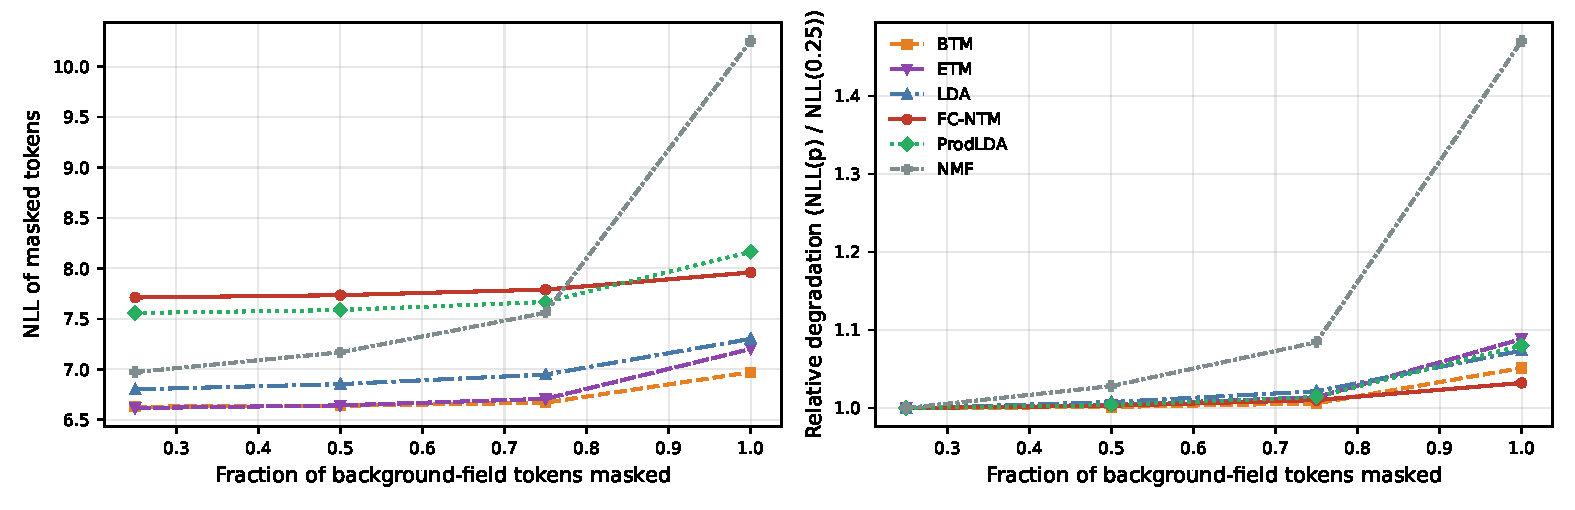
\includegraphics[width=0.86\textwidth]{fig_occlusion_en.pdf}
\caption{Inference behaviour under partial occlusion of the background field (GitHub issues,
seed 11, 2000 test documents). Left: per-token negative log-likelihood of the occluded tokens;
right: relative degradation $\mathrm{NLL}(p)/\mathrm{NLL}(0.25)$, which summarises the relative
increase from the 25\% condition without removing calibration differences. Line style and marker
identify the models, so the curves remain distinguishable in black-and-white print. \fcntm{} is trained
with whole-field dropout at $p=0.5$
and has the smallest relative degradation ($\times1.032$); the ratio itself cannot separate
``recovering content from the summary'' from ``being insensitive to the input'', and the absolute
NLL and agreement are not the best, as reported in the text.}
\label{fig:occlusion}
\end{figure}

\noindent\textbf{Cross-corpus comparison.} Table~S18 and Figure~S3 extend the same protocol to the three
corpora.

Three conclusions follow. First, the occlusion advantage is measured on only one of the three
corpora and does not follow the length ratio: on GitHub (ratio 12.9) all models degrade measurably
($\times1.028$--$\times1.470$) and \fcntm{} degrades least, beating the best baseline BTM by
$+0.024\pm0.004$ in the ten-seed paired comparison (10/10, $p=0.002$); on the civil corpus, whose
ratio is almost identical (11.2), \fcntm{} (1.010) leaves BTM marginally ahead on the same ratio (1.007 versus 1.010; paired difference $-0.003$, 0/10, $p=0.002$); on AG News (3.9) LDA remains the reference to beat (1.006 versus 1.019).
Second, no training-free statistic agrees with the three corpora: held-out mutual prediction is
slightly higher for GitHub, and the length ratio and background-exclusive share separate GitHub
from AG News but not from the civil corpus. Third, we therefore report these statistics as corpus
descriptions rather than as a pre-training criterion; establishing such a criterion requires
calibration on more corpora and an independent test corpus.

\noindent\textbf{Whole-field occlusion.} Deleting the background field entirely leaves topic-word coherence almost unchanged (all six cells
within $\pm0.02$, with sign flips across seeds on GitHub), so coherence is insensitive to field
loss and the information loss must be read from the document-level posterior and the word-level
prediction: about 66\% (GitHub) and 48\% (AG News) of the documents change their most probable
topic, and the per-token NLL rises by 0.24/0.23 with dropout training (0.24/0.27 without).
Training with whole-field dropout changes the shape of the posterior rather than the calibration of
word prediction: it lowers the per-token increase from 0.269 to 0.232 and the posterior JS from
0.060 to 0.049 on AG News, is directionally the same on the civil corpus
(0.125$\to$0.103, JS 0.039$\to$0.033), and shows no increase difference on GitHub
(0.242 versus 0.241) where only the JS slightly improves. Two corpora therefore show reduced
posterior drift under field loss, which cannot replace absolute prediction accuracy.

\noindent\textbf{Concatenated-field single-encoder control.} To compare the full method with a single-encoder alternative under the same budget we train a
control on the concatenated bag of words $[x_{\mathrm{bg}};x_{\mathrm{sm}}]$ with the same shared
linear decoder, field weights, KL warm-up and orthogonality penalty; whole-field dropout is
emulated by zeroing the background half of the input, and there is no fusion or consistency
term. The concatenated input doubles the first encoder layer, keeping the parameter count
comparable (a 1.5\% difference), and both models use the same budget, vocabulary and read-outs
on all three corpora (seeds 11/23/37).
Table~S19 reports the comparison.

The control is competitive everywhere, so the two-stream structure is not necessary for topic
quality. The mean difference favours \fcntm{} in every corpus--read-out cell ($+0.010$ to
$+0.029$ $C_V$), but the paired majorities are mixed (1/3 to 3/3) and the gaps are at the scale of
three-seed variation, so the two-stream architecture is a matched design choice rather than a
source of unconditional gains; the control also supports field-restricted read-out and title-only
inference.

\noindent\textbf{Title-only routing on the civil corpus.} When the abstract of a record is missing, can its title still be routed to an interpretable civil
subfield? The evaluation labels are the OpenAlex primary topics of each record --- external
automatic labels from a classifier rather than expert ground truth; the frozen snapshot (topic
IDs, fetch date) is released with the code, and the label set is the 15 most frequent topics of
the training split, covering 42.9\% of the test records (2000-record test split). Every model
infers a topic distribution from the title only (\fcntm{} and the control use their
missing-background inference path); the per-model topic-to-label mapping is a supervised step ---
the majority training label of each argmax topic, with the training-label prior as fallback for
topics that take no training record (three test records in one run triggered this fallback) ---
fitted on the same title-only inference, so the pipeline is an unsupervised representation with
a supervised training-split mapping. Accuracy and
macro-F1 are reported per seed; a supervised TF--IDF logistic regression on the same titles
serves as a reference point, and \fcntm{} with the full fields as an upper reference.
Table~S20 reports the accuracy and macro-F1 of each seed.

Topic-based routing from titles alone recovers a substantial part of the full-field signal
(0.664 versus 0.719 accuracy) and clearly outperforms the classical topic-model baselines
(LDA 0.532, BTM 0.600), but it remains well below a supervised TF--IDF classifier trained on the
same titles (0.810); the topic representation is learned without labels, while the topic-to-label
mapping uses training labels, which is why the supervised classifier retains its advantage. The
concatenated control reaches 0.653 against 0.664 for \fcntm{}, but the three paired per-seed
differences are not consistent in direction and the gap is small relative to the per-seed
variation, so the two architectures operate within comparable ranges on this task. The task
is a routing aid under a fixed label set, not a substitute for supervised classification, and
its accuracy depends on the 42.9\% label coverage of the 15-topic set.

\noindent\textbf{Ablations and field-restricted read-out.} The three-step fusion
ablation, the core-component ablation, the fusion-weight sensitivity and the field-restricted
read-out are reported in the Supplementary Material (Tables S9--S12), with the same protocol and
read-outs as the main tables.

The component ablations (the three-step fusion ablation and the
core-component ablation), the sensitivity sweep over the fusion-reconstruction weight, the
whole-field occlusion diagnostic, the field-redundancy measures and the field-restricted read-out
comparison are reported in the supplementary material (Tables S8--S13).

\section{Discussion and Limitations}

The reproducible part of dual-field topic modelling is the representation: one trained model
yields field-restricted topic words and still infers topic proportions when the background field is
missing (on GitHub about 66\% of the documents change their most probable topic and the per-token
NLL rises by 0.24). The advantage on generic coherence metrics is corpus-dependent: the ten-seed
comparison supports $+0.028$ $C_V$ over BTM on GitHub (9/10 seeds) and $+0.049$ on the civil corpus
(10/10), but $-0.009$ on AG News (3/10), and on the civil corpus the native $\beta$ read-out is also
above BTM ($+0.061$, 10/10). Coherence is sensitive to the decoding path, the training budget and
Monte-Carlo noise, and the held-out redundancy measures show that GitHub is slightly the more
predictable of the two corpora, so redundancy is reported as a description of the field relation
rather than as a predictor of the gain.

For engineering document management the field-restricted read-out matches how titles and
abstracts are written, the occlusion diagnostic corresponds to estimating topics when abstracts are
missing, and title-only routing maps such topics to civil subfields. These read-outs and the
concatenated-field control together show what the complete \fcntm{} configuration contributes.

\emph{Data extrapolation.} All three corpora are English and the field split follows existing
title/body structure; automatic field-boundary detection is untested, and the GitHub background field
has a long tail that the sentence-embedding baselines truncate at 128 tokens (the Supplementary Material
reports a window-pooling control). The conclusions therefore describe title/body-style records in
English. Extending them to other languages, other field conventions or automatically detected
boundaries requires re-running the same protocol on those corpora.

\emph{Experimental design.} The redundancy measures are computed on two corpora with almost the
same held-out predictability ($\rho^2_{\mathrm{cca}}$ 0.306 versus 0.245) while the ten-seed gain
appears on one of them, so the two corpora define the current calibration range; all numbers come
from one protocol ($K=30$, 700-epoch budget, unified read-out and evaluation vocabulary), with
\fcntm{} and BTM extended to ten seeds on all three corpora while the remaining baselines and the
main tables stay at three seeds. The precision of the reported comparisons is therefore bounded by
these seed counts, and a redundancy-based pre-training criterion or any claim outside these settings
requires calibration on additional corpora, more seeds for the remaining controls and an independent
confirmation corpus.

\emph{Method applicability.} Field-restricted read-out is available to any model with a
topic--word matrix and is not unique to a two-stream encoder; the non-parametric baselines choose
their own topic numbers and are shown for reference only; and the masking rate, the whole-field dropout
probability and the fusion weight are empirical values whose interaction with corpus size and field
ratio is not characterised. In addition, the in-house variational baselines and \fcntm{} use 20\% of the
training documents for early stopping (the official CombinedTM keeps its own held-out split), while
the class TF--IDF read-out of \fcntm{} aggregates the full training set, so the number of documents
used for optimisation and for read-out differs. The configuration reported here is therefore a
calibrated setting rather than a set of universal defaults, and transferring it should re-tune these
values on the target corpus.

\emph{Mechanism interpretation.} The concatenated-field control and the title-only routing task
are run for three seeds per cell and against one label source (OpenAlex primary topics), so their
differences should be read at the scale of the seed-to-seed variation; the occlusion ratio and the
redundancy measures describe, rather than predict, missing-field behaviour and the field relation.
Separating ``recovering content from the summary'' from ``insensitivity to the input'' therefore
requires a protocol with an independent source of the missing content.

\section{Summary and Conclusions}

This paper presented \fcntm{}, a field-cooperative neural topic model for dual-field short texts:
two conditional variational streams share one linear topic decoder, cross-field reconstruction and a
consistency regulariser encode the field relation into a shared topic space, and field-level word
masking and whole-field dropout handle partial and complete field absence. A single trained model
supports a decoder $\beta$ read-out and a class TF--IDF read-out under one evaluation vocabulary,
which removes the vocabulary and topic-length confounds of cross-model comparison.

On civil engineering title--abstract records and two public corpora the results depend on the
corpus. Under the read-out-matched protocol the ten-seed comparison gives $+0.028$ $C_V$ over BTM on
GitHub (95\% CI $[+0.012,+0.043]$, 9/10) and $-0.009$ on AG News (CI includes zero, 3/10); on the
civil corpus both read-outs favour \fcntm{} by a larger margin ($+0.049$ class TF--IDF and
$+0.061$ $\beta$, 10/10), and on the two public corpora BTM keeps its lead under the native $\beta$ read-out. A same-budget concatenated-field single encoder is close on every corpus (mean
$\Delta C_V$ $+0.010$--$+0.029$ with mixed paired majorities), and title-only routing reaches
0.66 accuracy against automatically assigned OpenAlex primary-topic labels on the 42.9\% of the test
split covered by the 15 selected topics. Taken together, the contributions are the field-cooperative configuration, the unified read-out
and the missing-field inference behaviour, with read-out-matched advantages supported by ten seeds on
the civil corpus and on GitHub. The boundaries of this evidence are stated by the two field-relation
measures: the corpora have similar redundancy, and occluding the background field leaves coherence
almost unchanged while changing the document-level posterior and the word-level prediction, so neither
measure is used to predict the direction of the gain. The complete configuration shows small mean
coherence gains over the concatenated control, and the reported effects are corpus-dependent;
whether field structure is worth the extra modelling cost should therefore be measured on the
target corpus with the protocol used here.

\section{Acknowledgments}

This work was supported by the National Key Research and Development Program of China under
Grant No. 2024YFC3809900, sub-project 2024YFC3809904-03 (``Research on Dynamic Investment
Control Models at the Transaction Stage''), undertaken at Harbin Institute of Technology.

\section{Data Availability Statement}

The code, the fixed corpus splits and the per-seed experimental results that support this study are
available at \url{https://github.com/wanghl0921/FCNTM}. The experiments can be reproduced with the
released configurations and evaluation scripts. Trained model checkpoints and the per-seed detail
dumps are released as assets of v1.0.0 in the same repository, and access to the third-party source
corpora remains subject to the terms and licences of the original providers.

\section{Practical Applications}

Engineering libraries and design offices accumulate far more title--abstract records than any team
can read one by one, and a large share of those records circulate with titles only. The method
presented here, FC-NTM, treats the title and the abstract of a record as two cooperating views of
the same subject: it learns one topic space for both fields and can still assign topics when the
abstract is missing. On the civil engineering corpus, FC-NTM achieved the highest topic coherence
among the evaluated methods. Its advantage over BTM was supported by ten paired random-seed
comparisons, while the comparisons with the other baselines followed the evaluation protocols
reported in the paper. A companion routing task shows
that titles alone can point to the right subject category for about two-thirds of the records
that carry an automatic category label, which supports browsing and screening rather than
replacing expert cataloguing. Because one trained model serves both a title-only and a
full-record reading, an organisation can index new records immediately and refine the index
later, when the abstract arrives. Collections that keep a short summary field beside a longer
descriptive field are the natural next setting in which to test the same procedure.

\section{Supplemental Materials}

The supplementary material (Tables S1--S20, Figures S1--S3, the ablation details and the training
details of the baselines) is available at
\url{https://github.com/wanghl0921/FCNTM/releases/download/v1.0.1/supplementary.pdf}.

% bibliography style is set by ascelike-new.cls
\bibliography{main_asce}

\end{document}
